\documentclass[12pt,a4paper,oneside]{book}
%\pagestyle{fancy}
%START OF PREAMBLE
\usepackage[english]{babel}
\usepackage{titlesec,xcolor,graphicx,color,soul,float}
\usepackage{blindtext,hyperref,fancyhdr,marginnote}
\usepackage[most]{tcolorbox}
\usepackage[scale=2,opacity=0.1,angle=0]{background}
\usepackage{float}

\hypersetup{
	colorlinks=true, 
	linkcolor=blue, 		
	filecolor=magenta, 
	urlcolor=cyan
}
\urlstyle{same}

\setlength\headheight{26pt}
\fancyhf{}
\lhead{\rightmark}
\rhead{\includegraphics[width=1cm]{logo}}

\fancyfoot[RE,RO]{\thepage}
\fancyfoot[CE,CO]{\href{http.//e-yantra.org}{www.e-yantra.org}}	

\titleformat{\chapter}
{\Large\bfseres}
{}
{0pt}
{\huge}

\tcbset{colback=cyan!5!white,colframe=cyan!75!black,halign title = flush center}

\newtcolorbox{mybox}[1]{colback=cyan!5!white,colframe=cyan!75!black,fonttitle=\bfseries,title=\textbf{\Large{#1}}}

\backgroundsetup{
contents={\includegraphics{logo}}
}

\newcommand{\keyword}[1]{\textcolor{red}{\textbf{#1}}}

\newcommand{\head}[1]{\textnormal{\textbf{#1}}}

%END OF PREAMBLE

%======================================================%
\begin{document}
	\begin{titlepage}
	\raggedright
	{\Large e-YSIP 2022\\[1cm]}
	{\Huge\scshape Self Balancing Robot Development \\[0.1in]}
	\vfill
	\begin{flushright}
		\textbf{{\begin{Large}Mentors\end{Large}}}\\
		Avijit Pandey\\
		Avinash Dubey\\
		Maddu Shravan Murali\\
		Amit Kumar\\
		
		\vspace{1cm}

		\textbf{{\begin{Large}Interns\end{Large}}}\\
		Kulasekaran\\
		Jaydev Yadav\\
		Aniruddha Thakre\\

		\vspace{1cm}
		
		\textbf{{\begin{Large}Duration of Internship\end{Large}}}\\
		$ 06/06/2022 - 05/08/2022 $
	\end{flushright}
	{\itshape 2022, e-Yantra Publication}
	\end{titlepage}
	
%======================================================%	
	
	\section*{Abstract}
		Spark interest and lessen the burden in learning/Explaining the concepts of Control systems / Robotics / Embedded systems among students, Hobbyist, Kids, Teachers and Professors.  and so to develop a Self Balancing robot which can be assembled from a kit and can also act as a toy. 
		\subsection*{Completion Status}
		The work began with conducting market surveys to find similar products online and conducting interviews among various user personas to get their views and so to categorize the needs and wants. After that, CAD designing of the bot was carried out and completed. The necessary parts were procured, laser cut and 3D printed and the bot has been fabricated fully. PCB designing and wiring has also been done and the PID values have been tuned to make the bot balance itself.

%======================================================%
		
	\section*{Hardware Parts}
		\begin{table}[H]
		\def\arraystretch{1.5}
		\caption{\textbf{List of Hardware Components}}
		\vspace{1cm}
		\begin{tabular}{|c|c|c||c|c|c|}
			\hline
			\textbf{Sl.No} & \textbf{Component} & \textbf{Qty} & \textbf{Sl.No} & \textbf{Component} & \textbf{Qty}\\\hline
			1. & eYFI Board & 1 & 15. & Extension PCB & 1 \\\hline
			2. & Deadweight & 1 & 16. & Motors & 2 \\\hline
			3. & 85mm Wheels & 2 & 17. & GearBox & 2 \\\hline
			4. & 8-array Line Sensor & 1 & 18. & Battery & 1 \\\hline
			5. & Large Bearing & 2 & 19. & Small Bearing & 8 \\\hline
			6. & Hercules Motor Driver & 2 & 20. & Lid for Gearbox & 2 \\\hline
			7. & Height Adjusting Gears & 2 & 21. & Castor Wheels & 2 \\\hline
			8. & LeadScrew & 1 & 22. & 14.5cm Spacers & 4 \\\hline
			9. & HC-Sr04 Ultrasonic Sensor & 1 & 23. & OV7670 Camera & 1 \\\hline
			10. & 1.3" OLED & 2 & 24. & GY87 Gyro Sensor & 1 \\\hline
			11. & Driver Gear & 2 & 25. & Driven Gear & 2 \\\hline
			12. & IR-Obstacle Sensor & 4 & 26. & 1cm Spacers & 4 \\\hline
			13. & 4cm Spacers & 4 & 27. & 5cm Spacers & 4 \\\hline
			14. & Cover-Back & 1 & 28. & Cover-Front & 1 \\\hline
			15. & Cover-Bottom & 1 & 29. & Acrylic Plates & 5 \\\hline			
		\end{tabular}
		\end{table}
		\pagebreak

		\subsection*{Details of each Hardware}
			\subsubsection*{1. eYFI Board}
				\begin{figure}[H]
					\centering					
					\includegraphics[scale=1]{EYFI FULL}
					\caption{eYFI board with Extension board}	 
				\end{figure}
				\begin{table}[H]
					\centering
					\def\arraystretch{1.2}
					\caption{eYFI board details}
					\vspace{0.5cm}
					\begin{tabular}{|c||c|}
					\hline
						\textbf{eYFI Dimensions(L*W*H)} & 6.4cm * 1.7cm * 11cm\\\hline
						\textbf{Extension PCB Dimensions(L*W*H)} & 14cm * 0.2cm * 15cm\\\hline
						\textbf{Programming Mode} & USB/OTA\\\hline
						\textbf{Microcontroller} & ATmega2560 \& ESP32\\\hline
						\textbf{Operating Voltage(ATmega2560)} & 5 V\\\hline 
						\textbf{Operating Voltage(ESP32)} & 3.3 V\\\hline 
						\textbf{INPUT VOLTAGE (RECOMMENDED)} & 7V - 12V\\\hline
						\textbf{INPUT VOLTAGE (LIMIT)} & 6V - 20V\\\hline
					\end{tabular}
				\end{table}
				\pagebreak
				
			\subsubsection*{2. 85mm Wheel}
				\begin{figure}[H]
					\centering
					\includegraphics[scale=1]{Wheel FULL}
					\caption{85mm Wheel}	 
				\end{figure}
				\begin{table}[H]
					\centering
					\def\arraystretch{1.2}
					\caption{85mm Wheel details}
					\vspace{0.5cm}
					\begin{tabular}{|c||c|}
					\hline
						\textbf{Dimensions(L*W*H)} & 8.5cm * 3cm * 8.5cm\\\hline
						\textbf{Material}  & Rubber \& Plastic\\\hline
						\textbf{Link to Buy} & \href{https://robu.in/product/85mm-large-robot-smart-car-wheel-38mm-width-surface-blue/}{85mmWheel@Robu.in}\\\hline
					\end{tabular}
				\end{table}
				\pagebreak
				
			\subsubsection*{3. GearBox}
				\begin{figure}[H]
					\centering					
					\includegraphics[scale=1]{GEARBOX FULL}
					\caption{Gearbox}	 
				\end{figure}
				\begin{table}[H]
					\centering
					\def\arraystretch{1.5}
					\caption{Gear Box Details}
					\vspace{0.5cm}
					\begin{tabular}{|c||c|}
					\hline
						\textbf{Dimensions(L*W*H)} & 7.5cm * 3.6cm * 6cm\\\hline
						\textbf{Material} & Polylactic acid(PLA) (3D printed)\\\hline
						\textbf{Small Hole Dia} & 1.75cm\\\hline
						\textbf{Large Hole Dia}	& 2.15cm\\\hline
						\textbf{Screw Hole Dia} & 0.4cm\\\hline
					\end{tabular}
				\end{table}
				\pagebreak
				
			\subsubsection*{4. 8-array Line Sensor}
				\begin{figure}[H]
					\centering					
					\includegraphics[scale=1]{LINE SENSOR FULL}
					\caption{8-Array Line Sensor}	 
				\end{figure}
				\begin{table}[H]
					\centering
					\def\arraystretch{1.5}
					\caption{Line Sensor Details}
					\vspace{0.5cm}
					\begin{tabular}{|c||c|}
					\hline
						\textbf{Dimensions(L*W*H)} & 10cm * 2.8cm * 1.3cm\\\hline
						\textbf{No. of Photodiode} & 8\\\hline
						\textbf{Input Voltage} & 5V\\\hline
						\textbf{Communication Protocol} & I2C\\\hline
						\textbf{Link to Buy} & \href{https://products.e-yantra.org/eylfa/}{Products @ eyantra}\\\hline
					\end{tabular}
				\end{table}
				\pagebreak
				
			\subsubsection*{5. Battery}
				\begin{figure}[H]
					\centering					
					\includegraphics[scale=1]{BATTERY FULL}
					\caption{2200mah battery}	 
				\end{figure}
				\begin{table}[H]
					\centering
					\def\arraystretch{1.5}
					\caption{Battery Details}
					\vspace{0.5cm}
					\begin{tabular}{|c||c|}
						\hline
						\textbf{Dimensions(L*W*H)} & 6.5cm * 3.5cm * 3cm\\\hline
						\textbf{Current capacity} & 1300mah\\\hline
						\textbf{Voltage capacity} & 11.1 V\\\hline
						\textbf{Link to Buy} & \href{https://robu.in/product/orange-1300mah-4s-100c200c-lithium-polymer-battery-pack-lipo/}{Robu.in}\\\hline
					\end{tabular}
				\end{table}
				\pagebreak
				
			\subsubsection*{6. Bearing}
				\begin{figure}[H]
					\centering
					\includegraphics[scale=1]{BEARING}
					\caption{Large \& Small Bearings}	 
				\end{figure}
				\begin{table}[H]
					\centering
					\def\arraystretch{1.5}
					\caption{Bearing Details}
					\vspace{0.5cm}
					\begin{tabular}{|c||c|}
						\hline
						\multicolumn{2}{|c|}{Large Bearing}\\\hline
						\textbf{Dimensions(L*W*H)} & 3.4cm * 1cm * 3.4cm\\\hline
						\textbf{Inner Dia} & 1.5cm\\\hline
						\multicolumn{2}{|c|}{Small Bearing}\\\hline						
						\textbf{Dimensions(L*W*H)} & 1.6cm * 0.5cm * 1.6cm\\\hline
						\textbf{Inner Dia} & 0.6cm\\\hline 
						\textbf{Link to Buy} & \href{https://omrook.com/bearing/ball-bearing/series-6200/6202-zz-id-15mm-od-35mm-deep-groove-ball-bearing-15x35x11/?gclid=CjwKCAjw6fyXBhBgEiwAhhiZsknjuPBmqFP17BJH1Lhju9C-yQazRN_64urzpzRYuYJUoWjsgJFw3RoCs8wQAvD_BwE}{Large Bearing}\\\hline
						\textbf{Link to Buy} & \href{https://robu.in/product/696zz-bearing-6x15x5-stainless-steel-shielded-miniature-bearings-4pcs/}{SmallBearing @ Robu.in}\\\hline
					\end{tabular}
				\end{table}
				\pagebreak
				
			\subsubsection*{7. Hercules Motor Driver}
				\begin{figure}[H]
					\centering
					\includegraphics[scale=1]{MOTOR DRIVER FULL}
					\caption{Hercules Motor Driver}	 
				\end{figure}
				\begin{table}[H]
				\centering
				\def\arraystretch{1.5}
					\caption{Motor Driver Details}
					\vspace{0.5cm}
					\begin{tabular}{|c||c|}
					\hline
						\textbf{Dimensions(L*W*H)} & 7.1cm * 2.5cm * 3.65cm\\\hline
						\textbf{Logic Input Voltage (Recommended)} & 5 V\\\hline
						\textbf{Operating Voltage (Recommended)} & 12 V\\\hline
						\textbf{Operating Voltage (Limit)} & 6 V - 36 V\\\hline
						\textbf{Link to Buy} & \href{http://www.nex-robotics.com/products/motor-drivers/hercules-6v-36v-16amp-motor-driver.html}{@NexRobotics}\\\hline
					\end{tabular}
				\end{table}
				\pagebreak
				
			\subsubsection*{8. Driver and Driven Gears}
				\begin{figure}[H]
					\centering
					\includegraphics[scale=0.6]{DRIVER AND DRIVEN GEAR}
					\caption{Driver and Driven gears}	 
				\end{figure}
				\begin{table}[H]
				\centering
				\def\arraystretch{1.5}
					\caption{Driver and Driven Gear Details}
					\vspace{0.5cm}
					\begin{tabular}{|c||c|c|}
					\hline
					\textbf{} & \textbf{Driver gear} & \textbf{Driven gear}\\\hline
					\textbf{Num of Teeth} & 20 & 40\\\hline
					\textbf{Addendum dia} & 2.2cm & 4.2cm\\\hline
					\textbf{Pitch circle Dia} & 1.96cm & 4cm\\\hline
					\textbf{Deddendum Dia} & 1.78cm & 3.72cm\\\hline
					\textbf{Large shaft dia} & 1.15 & 1.4cm\\\hline
					\textbf{small shaft dia} & 0.56 & 0.56cm\\\hline
					\textbf{Module} & \multicolumn{2}{|c|}{1mm}\\\hline
					\textbf{Face width} & \multicolumn{2}{|c|}{0.5cm}\\\hline
					\textbf{Gear Ratio} & \multicolumn{2}{|c|}{2:1}\\\hline
					\end{tabular}
				\end{table}
				\pagebreak
				
			\subsubsection*{9. Height Adjusting Gears}
				\begin{figure}[H]
					\centering					
					\includegraphics[scale=0.8]{H_ADJUST GEARS FULL}
					\caption{Height Adjusting Gears}	 
				\end{figure}
				\begin{table}[H]
				\centering
				\def\arraystretch{1.5}
					\caption{Height Adjusting Gear Details}
					\vspace{0.5cm}
					\begin{tabular}{|c||c|c|}
					\hline
						\textbf{} & \textbf{Main Gear} & \textbf{Side Gear}\\\hline
						\textbf{Num of Teeth} & 30 & 30\\\hline
						\textbf{Addendum Dia} & 6.4cm & 6.4cm\\\hline
						\textbf{Pitch Circle Dia} & 5.98cm & 5.98cm\\\hline
						\textbf{Dedenum Dia} & 5.6cm & 5.6cm\\\hline
						\textbf{Face Width} & 0.5cm & 0.5cm\\\hline
						\textbf{Shaft Dia} & . & 0.56cm\\\hline
						\textbf{Material} & \multicolumn{2}{|c|}{Polylactic acid (PLA)}\\\hline
						\textbf{Module} & \multicolumn{2}{|c|}{2mm}\\\hline
						\textbf{Gear Ratio} & \multicolumn{2}{|c|}{2:1}\\\hline
					\end{tabular}
				\end{table}
				\pagebreak
				
			\subsubsection*{10. Castor Wheels}
				\begin{figure}[H]
					\centering					
					\includegraphics[scale=1]{CASTOR FULL}
					\caption{Castor wheels}	 
				\end{figure}
				\begin{table}[H]
				\centering
				\def\arraystretch{1.5}
					\caption{Castor Wheel Details}
					\vspace{0.5cm}
					\begin{tabular}{|c||c|}
					\hline
						\textbf{Base Dia} & 2.7cm\\\hline
						\textbf{Screw Hole Dia} & 0.4cm\\\hline
						\textbf{Ball Dia} & 1.36cm\\\hline
						\textbf{Height} & 1.9cm\\\hline
						\textbf{Material} & Metal\\\hline
						\textbf{Link to Buy} & \href{https://www.electroncomponents.com/Caster-wheel-robot-center-metal-ball-24mm}{@Electron Components}\\\hline
					\end{tabular}
				\end{table}
				\pagebreak
				
			\subsubsection*{11. LeadScrew}
				\begin{figure}[H]
					\centering					
					\includegraphics[scale=1]{LEADSCREW}
					\caption{LeadScrew for adjusting dead weight}	 
				\end{figure}
				\begin{table}[H]
				\centering
				\def\arraystretch{1.5}
					\caption{LeadScrew Details}
					\vspace{0.5cm}
					\begin{tabular}{|c||c|}
					\hline
						\textbf{Length} & 15cm\\\hline
						\textbf{Diameter} & 0.78cm\\\hline
						\textbf{Material} & Metal\\\hline
					\end{tabular}
				\end{table}
				\pagebreak
			
			\subsubsection*{12. Spacers}
				\begin{figure}[H]
					\centering					
					\includegraphics[scale=1]{SPACERS TOP}
					\caption{Spacers of different lengths}	 
				\end{figure}
				\begin{table}[H]
				\centering
				\def\arraystretch{1.5}
					\caption{Spacer Details}
					\vspace{0.5cm}
					\begin{tabular}{|c||p{5cm}|}
					\hline
						\textbf{Lengths of Spacers} & 1cm Spacer, 4cm Spacer, 5cm Spacer, 14.5cm Spacer\\\hline
						\textbf{Link to Buy} & \href{https://robu.in/product/m310mm-male-to-female-nylon-hex-spacer-10pcs-copy/}{1cm Spacer}\\\hline
						\textbf{Link to Buy} & \href{https://www.electronicscomp.com/m3-x-40mm-male-to-female-brass-hex-threaded-pillar-standoff-spacer-2-pieces-pack?gclid=CjwKCAjw6fyXBhBgEiwAhhiZsguSTtz-rwfcqkDPwz9-GVv6AfvZXK3TcJzOwtoXo6S8MNRfq46vxRoCE0cQAvD_BwE}{4cm Spacer}\\\hline
						\textbf{Link to Buy} & \href{https://www.electronicscomp.com/metal-spacer-50mm-male-female?gclid=CjwKCAjw6fyXBhBgEiwAhhiZsux4DW3Xj_j21q39Tm3qviNldIP9u2m_7gQ3t3tbwMVXk955l_NgthoCCBkQAvD_BwE}{5cm Spacer}\\\hline
						\textbf{Link to Buy} & \href{???}{14.5cm Spacer (???)}\\\hline
					\end{tabular}
				\end{table}
				\pagebreak
				
			\subsubsection*{13. HC-Sr04 Ultrasonic Sensor}
				\begin{figure}[H]
					\centering					
					\includegraphics[scale=1]{ULTRASONIC FULL}
					\caption{HC-SR04 Ultrasonic sensor}	 
				\end{figure}
				\begin{table}[H]
				\centering
				\def\arraystretch{1.5}
					\caption{Ultrasonic Sensor Details}
					\vspace{0.5cm}
					\begin{tabular}{|c||c|}
					\hline
						\textbf{Dimensions(L*W*H)} & 4.57cm * 1.7cm * 2.63cm\\\hline
						\textbf{Pins} & 4\\\hline
						\textbf{Input Voltage} & 5 V\\\hline
						\textbf{Link to Buy} & \href{https://robu.in/product/hc-sr04-ultrasonic-range-finder/}{@Robu.in}\\\hline
					\end{tabular}
				\end{table}
				\pagebreak
				
			\subsubsection*{14. OV7670 Camera}
				\begin{figure}[H]
					\centering
					\includegraphics[scale=1]{CAM FULL}
					\caption{OV7670 Camera module}	 
				\end{figure}
				\begin{table}[H]
				\centering
				\def\arraystretch{1.5}
					\caption{Camera module Details}
					\vspace{0.5cm}
					\begin{tabular}{|c||c|}
					\hline
						\textbf{Dimension(L*W*H)} & 3.5cm * 3cm * 4cm\\\hline
						\textbf{Pins} & 18\\\hline
						\textbf{Input Voltage} & 3.3 V\\\hline
						\textbf{Link to Buy} & \href{https://robu.in/product/ov7670-640x480-vga-cmos-camera-image-sensor-module/}{@Robu.in}\\\hline
					\end{tabular}
				\end{table}
				\pagebreak
				
			\subsubsection*{15. 1.3" OLED display}
				\begin{figure}[H]
					\centering					
					\includegraphics[scale=1]{oled_front}
					\caption{1.3" OLED Displays}	 
				\end{figure}
				\begin{table}[H]
				\centering
				\def\arraystretch{1.5}
					\caption{OLED Details}
					\vspace{0.5cm}
					\begin{tabular}{|c||c|}
						\hline
						\textbf{Dimensions(L*W*H)} & 3.5cm * 0.8cm * 3.3cm\\\hline
						\textbf{Pins} & 4\\\hline
						\textbf{Input Voltage} & 5 V\\\hline
						\textbf{Link to Buy} & \href{https://robu.in/product/1-3-inch-i2c-iic-oled-lcd-module-4pin-with-vcc-gnd-white/}{@Robu.in}\\\hline
					\end{tabular}
				\end{table}
				\pagebreak
				
			\subsubsection*{16. GY87 Gyro Sensor}
				\begin{figure}[H]
					\centering
					\includegraphics[scale=0.7]{GYRO ISO}
					\caption{GY87 Gyro Sensor}	 
				\end{figure}
				\begin{table}[H]
				\centering
				\def\arraystretch{1.5}
					\caption{Gyro Sensor Details}
					\vspace{0.5cm}
					\begin{tabular}{|c||c|}
						\hline
						\textbf{Dimensions(L*W*H)} & 1.5cm * 0.2cm * 2.0cm\\\hline
						\textbf{Pins} & 8\\\hline
						\textbf{Input Voltage} & 5 V\\\hline
						\textbf{Communication Protocol} &  I2C\\\hline
						\textbf{Link to Buy} & \href{https://robu.in/product/mpu6050hmc5883lbmp180-10dof-3-axis-gyro-3-axis-acceleration-3-axis-magnetic-field-air-pres/}{@Robu.in}\\\hline
					\end{tabular}
				\end{table}
				\pagebreak
				
			\subsubsection*{17. IR-Obstacle Sensor}
				\begin{figure}[H]
					\centering
					\includegraphics[scale=1]{IR FULL}
					\caption{IR-Obstacle sensor}	 
				\end{figure}
				\begin{table}[H]
				\centering
				\def\arraystretch{1.5}
					\caption{IR Sensor Details}
					\vspace{0.5cm}
					\begin{tabular}{|c||c|}
						\hline
						\textbf{Dimensions(L*W*H)} & 4.45cm * 1.36cm * 1.914cm\\\hline
						\textbf{Pins} & 3\\\hline
						\textbf{Input Voltage} & 5 V\\\hline
						\textbf{Link to Buy} & \href{https://robu.in/product/sharp-ir-distance-measuring-sensor-unit-4-30-cm-cable/}{@Robu.in}\\\hline
					\end{tabular}
				\end{table}
				\pagebreak
				
			\subsubsection*{18. Cover}
				\begin{figure}[H]
					\centering
					\includegraphics[scale=1.2]{COVER FULL}
					\caption{A Three Part cover for easier accessibility}	 
				\end{figure}
				\begin{table}[H]
				\centering
				\def\arraystretch{1.5}
					\caption{Cover Details}
					\vspace{0.5cm}
					\begin{tabular}{|c||c|}
						\hline
						\multicolumn{2}{|c|}{\textit{Front Cover}}\\\hline
						\textbf{Dimensions(L*W*H)} & 20.78cm * 9cm * 18.8cm\\\hline
						\multicolumn{2}{|c|}{\textit{Back Cover}}\\\hline					
						\textbf{Dimensions(L*W*H)} & 20.78cm * 9cm * 18.8cm\\\hline
						\multicolumn{2}{|c|}{\textit{Bottom Cover}}\\\hline				
						\textbf{Dimensions(L*W*H)} & 20.61cm * 18cm * 10.5cm\\\hline
						\textbf{Material} & acid(PLA)\\\hline
					\end{tabular}
				\end{table}
				\pagebreak
			
			\subsubsection*{19. Acrylic Plates}
				\begin{center}
					\begin{figure}[H]
						\includegraphics[scale=1]{PLATES FULL}
						\caption{Acrylic Plates}	 
					\end{figure}
				\end{center}
				\begin{table}[H]
				\centering
				\def\arraystretch{1.5}
					\caption{Acrylic Plate Details}
					\vspace{0.5cm}
					\begin{tabular}{|c||c|}
						\hline
						\textbf{Material} & Acrylic\\\hline
						\textbf{Thickness} & 5mm\\\hline
						\textbf{Quantity} & 5\\\hline						
					\end{tabular}
				\end{table}
				\pagebreak
			
		\subsection*{Connection Diagram}
			\begin{huge}
				\textit{JAYDEV'S WORK}
			\end{huge}
			\pagebreak
			

%======================================================%
		%JAYDEV'S WORK
	\section*{Software used}
		\subsection*{List of Software used}
			\begin{itemize}
				\item \href{https://www.arduino.cc/en/software}{Arduino IDE}
				\item \href{https://www.solidworks.com/sw/support/downloads.htm}{Solidworks 2022}
			    \item \href{https://www.keyshot.com/direct-downloads/}{Keyshot 11}
			\end{itemize}
			\pagebreak
			
            \begin{huge}
                \textbf{Environment setup instructions}
            \end{huge}
            \begin{itemize}
                \item Adding EYFi Mega to Arduino IDE
            \end{itemize}
  
            \begin{enumerate}
                \item  Open Preferences
                    \begin{itemize}
                        \item Files $\to$ Preferences
                    \end{itemize}
                \item Click on the button to the right of the Additional Boards Manager URLs text field.
                \item Paste or Remove URLs in the window. There should be one URL for each line.
                \begin{center}
    				\includegraphics[scale=0.85]{Preference}
    			\end{center} 
    			\item Links to be added are given Below :
                    \begin{itemize}
                        \item \href{https://raw.githubusercontent.com/eYSIP-2020/eysip2020-36-eYFi-Mega-ArduinoIDE/master/e-Yantra-ESP32/eYFi-Mega%20board/package_eyantra_eYFi-Mega-ESP32_index.json}{Adding eYFi Mega-ESP32 to Arduino IDE}
                         \item \href{https://raw.githubusercontent.com/eYSIP-2020/eysip2020-36-eYFi-Mega-ArduinoIDE/master/e-Yantra-ATmega2560/eYFi-Mega%20board/package_eyantra_eYFi-Mega-Atmega2560_index.json, https://raw.githubusercontent.com/eYSIP-2020/eysip2020-36-eYFi-Mega-ArduinoIDE/master/e-Yantra-ATmega2560/eYFi-Mega%20board/package_eyantra_eYFi-Mega-Atmega2560_index.json}{Adding eYFi Mega-Atmega2560 to Arduino IDE}
                    \end{itemize}  
                 \item Click OK.
                 \item Click OK in Preferences to save the changes.
                 \item Then go to Tools $\to$ Board $\to$ Boards Manager and search eYFi \newline and install both available options
                \begin{center}
                    \includegraphics[scale=0.85]{BOARDS MANAGER}
                \end{center}
                \item Now eYFi Mega Boards are being added to Arduino IDE
            \end{enumerate}
    \pagebreak

%======================================================%
    \begin{huge}
    \textbf{Flashing Code on eYFI Mega}
    \end{huge}
    \begin{enumerate}
        \item Go to Tools then Boards
        \item Select eYFi-Mega Atmega2560 Section
        \item Select eYFi-Mega(Atmega2560 Section)
            \begin{center}
            \includegraphics[scale=0.4]{SELECTING EYFI BOARD.png}
            \end{center}
        \item Select Disabled if Flashing the code through wired connection
        \item Select Upload \& Flash if Flashing the code using Wifi.
        \begin{center}
            \includegraphics[scale=0.6]{eYFi OTA.png}
        \end{center}
    \end{enumerate}
    

    \pagebreak
		
%======================================================%
		
	\section*{Assembly of Hardware}
		\subsubsection*{Connections}
			\begin{figure}[H]
				\begin{center}
					\includegraphics[scale=0.45]{PCB_FRONT_SIDE_1}
					\caption{Connectors}
				\end{center}
			\end{figure}
			\begin{itemize}
				\item Above Picture is positioning all the different types of peripheral Pins and GPIO of EYFI Mega. 
			\end{itemize}

			\begin{figure}[H]
				\begin{center}
					\includegraphics[scale=0.45]{PCB_FRONT_SIDE_2}
					\caption{Pinheaders}
				\end{center}
			\end{figure}
			\begin{itemize}
				\item Above Picture is positioning headers of different Sensors/Actuators. 
			\end{itemize}

			\begin{figure}[H]
				\begin{center}
					\includegraphics[scale=0.45]{PCB_BACK_SIDE_1}
					\caption{Pinheaders}
				\end{center}
			\end{figure}
			\begin{itemize}
				\item Above Picture is positioning headers of different Sensors/Actuators. 
			\end{itemize}
			
			\pagebreak

			\subsection*{Connection diagrams}
		
		\subsubsection*{STEP 1}
				\begin{figure}[H]
					\begin{center}
						\includegraphics[scale=0.50]{Motor_Hercules_Connection}
						\caption{Rhino Motor, Hercules Motor Driver and Board Connection}
					\end{center}
				\end{figure}
				\begin{itemize}
					\item To connect motor to Hercules motor driver and Board follow this connection diagram.
					\item M1 = Motor 1 and M2 = Motor 2
				\end{itemize}

		\subsubsection*{STEP 2}
				\begin{figure}[H]
					\begin{center}
						\includegraphics[scale=0.50]{Battery_Connection}
						\caption{Battery and Board Connection}
					\end{center}
				\end{figure}
				\begin{itemize}
					\item Follow above connection diagram to connect Battery to board.
				\end{itemize}

		\subsubsection*{STEP 3}
				\begin{figure}[H]
					\begin{center}
						\includegraphics[scale=0.50]{LineFollower_connection}
						\caption{Line follower and board connection}
					\end{center}
				\end{figure}
				\begin{itemize}
					\item Follow above connection diagram to connect line follower sensor and board.
				\end{itemize}

		\subsubsection*{STEP 4}
				\begin{figure}[H]
					\begin{center}
						\includegraphics[scale=0.50]{OLED_Connection}
						\caption{OLED display and board connection}
					\end{center}
				\end{figure}
				\begin{itemize}
					\item Follow above connection diagram to connect Oled Display and board.
				\end{itemize}

		\subsubsection*{STEP 5}
				\begin{figure}[H]
					\begin{center}
						\includegraphics[scale=0.50]{Ultrasonic_connection}
						\caption{Ultrasonic Sensor and board connection}
					\end{center}
				\end{figure}
				\begin{itemize}
					\item Follow above connection diagram to connect Ultrasonic Sensor and board.
				\end{itemize}

		\subsubsection*{STEP 6}
				\begin{figure}[H]
					\begin{center}
						\includegraphics[scale=0.50]{Camera_connection}
						\caption{Camera and board connection}
					\end{center}
				\end{figure}
				\begin{itemize}
					\item Follow above connection diagram to connect camera and board.
				\end{itemize}

		
		\pagebreak
		
		\subsection*{Assembly Instructions}
			\subsubsection*{STEP 1}
				\begin{figure}[H]
					\begin{center}
						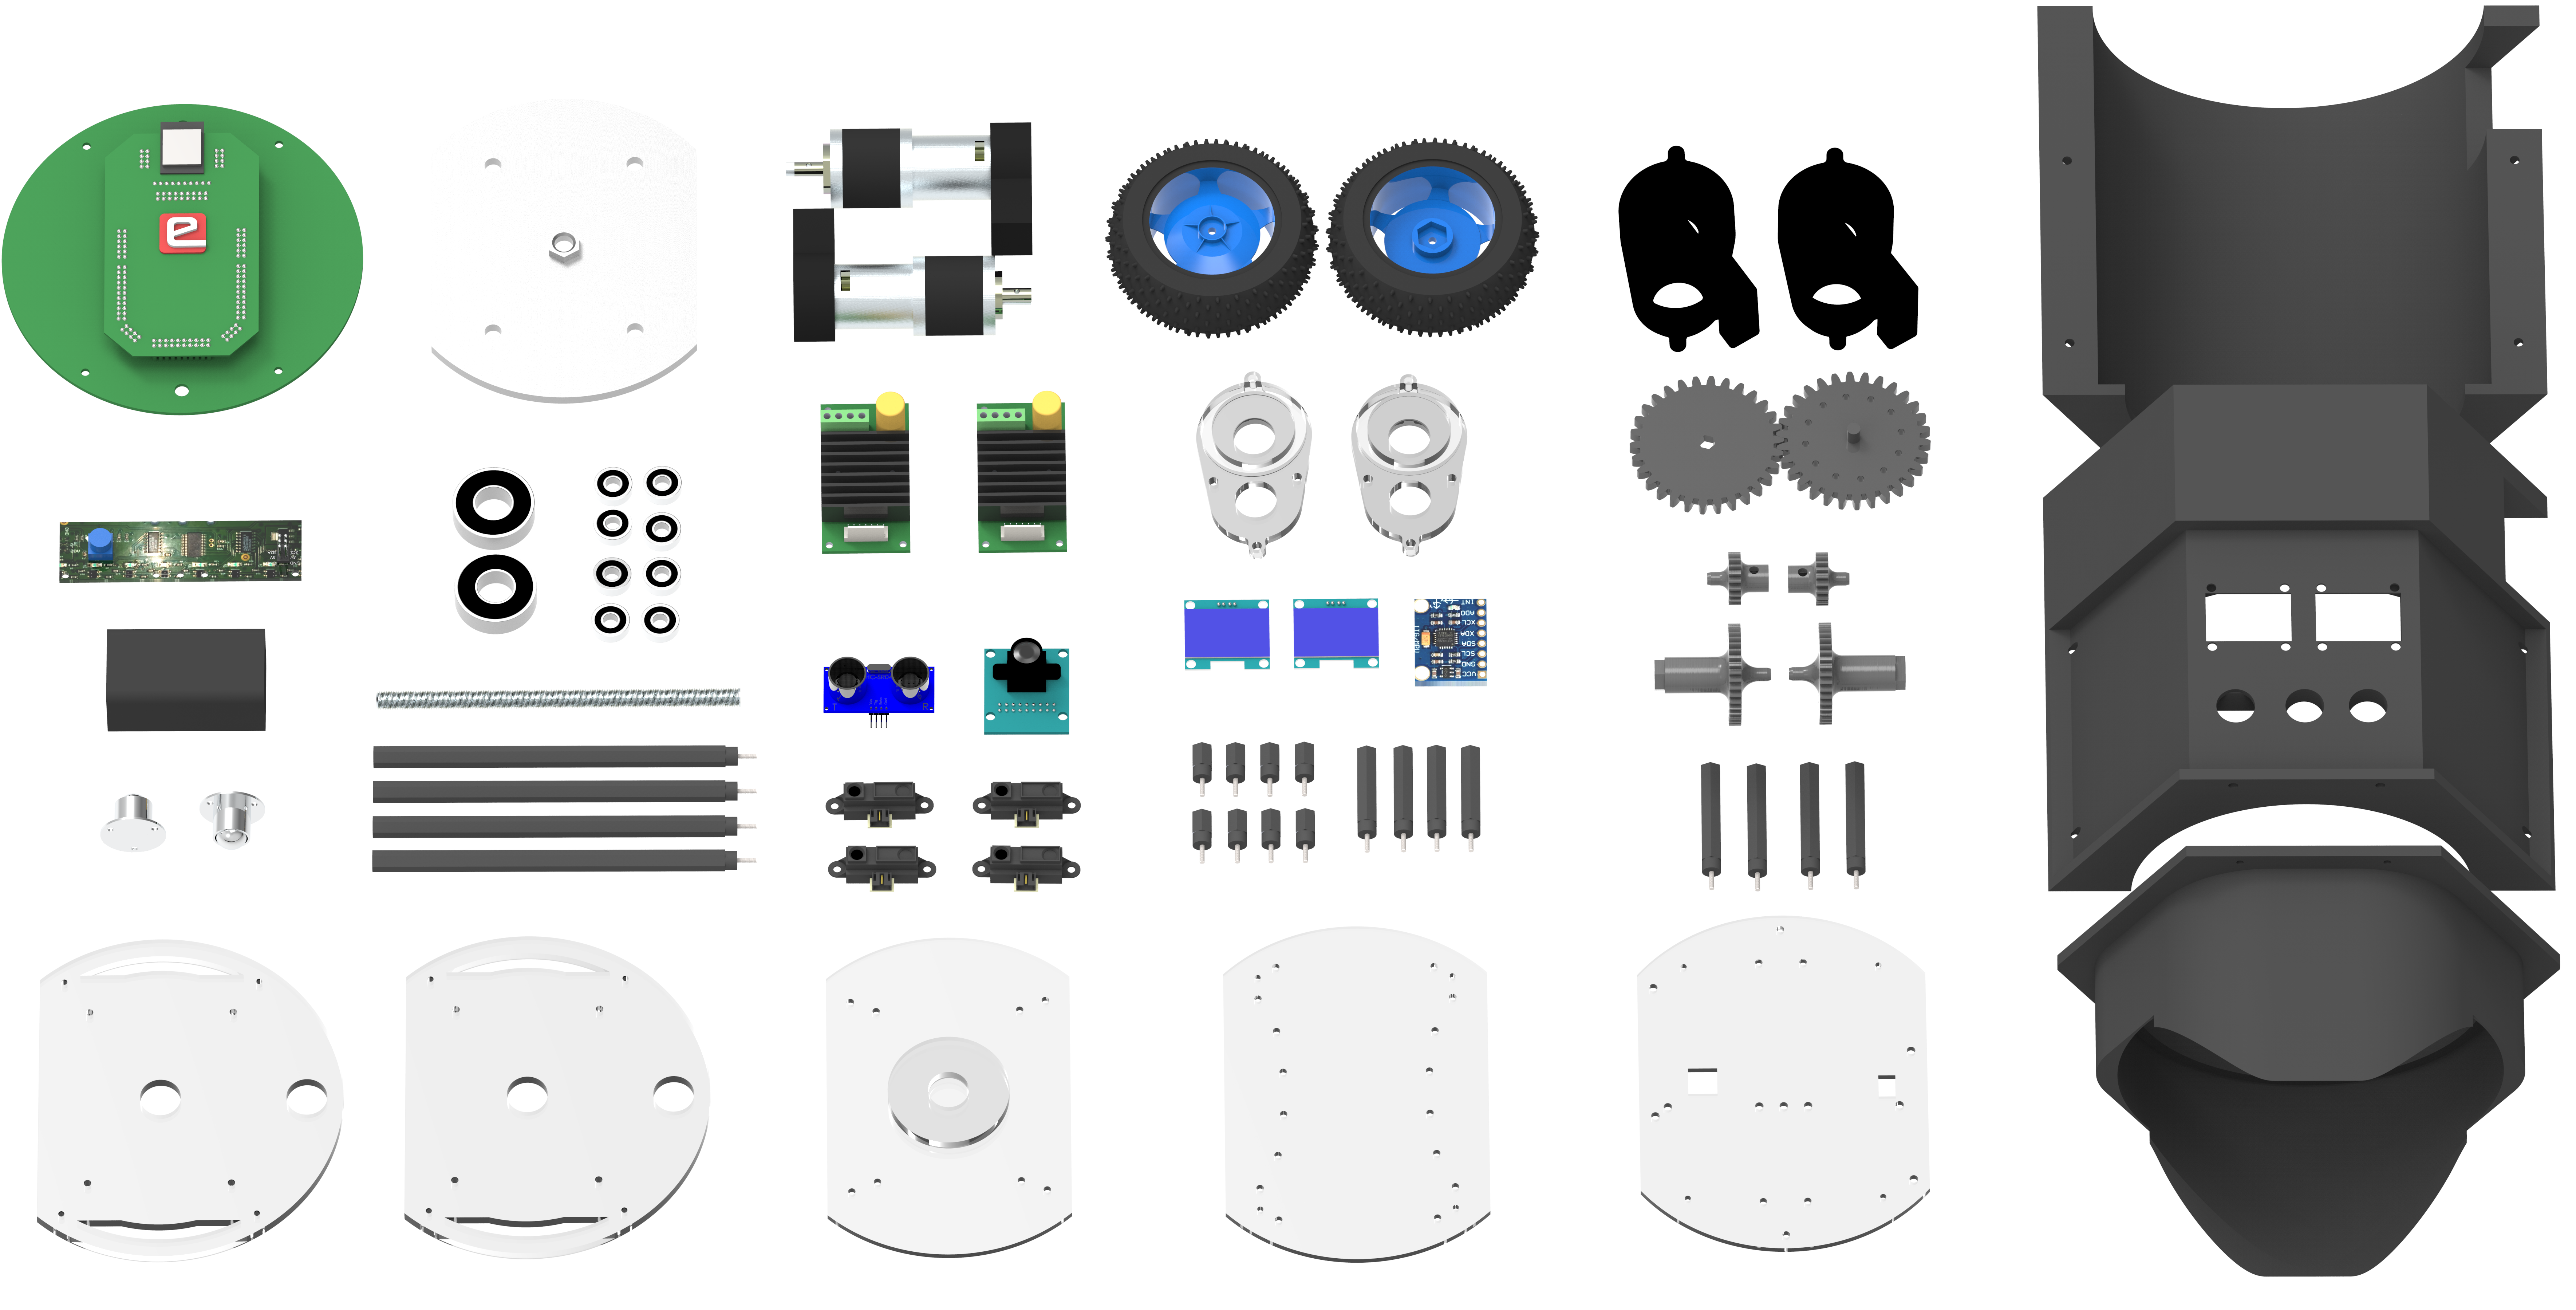
\includegraphics[scale=0.25]{Components}
						\caption{What you get in the box}
					\end{center}
				\end{figure}
				\begin{itemize}
					\item Before starting the assembly process, make sure that all the components are present to begin with and arrange them as shown in the Figure for easier identification. 
				\end{itemize}
				
				
			\subsubsection*{STEP 2}
				\begin{figure}[H]
					\begin{center}
						\includegraphics[scale=0.75]{BASEPLATE MARKED}
						\caption{Base plate}
					\end{center}
				\end{figure}
				\begin{itemize}
					\item First, identify the Base plate among the components. Carefully take note of which hole is to fit what from the illustration shown above in \textbf{Fig.20}
				\end{itemize}
				\pagebreak

			\subsubsection*{STEP 3}
				\begin{figure}[H]
					\begin{center}
						\includegraphics[scale=0.55]{ATTACHING LINE SENSOR}
						\caption{Attaching Line Sensor with Base plate}
					\end{center}
				\end{figure}
				\begin{itemize}
					\item Carefully attach the Line sensor to the bottom of the base plate and lock it with M3 nuts and bolts
					\item Now, the next step is to make the gear box assembly ready before attaching it to the Baseplate
				\end{itemize}
				
			\subsubsection*{STEP 4}
				\begin{figure}[H]
					\begin{center}
						\includegraphics[scale=0.65]{ATTACHING MOTOR TO GEARBOX}
						\caption{Attaching Motor to Gearbox}
					\end{center}
					\begin{itemize}
						\item Fix the motor as exactly shown in the \textbf{fig.22}, as it is very important. Note that the black color cap in the back of the motor should be facing the direction as shown in \textbf{fig.22}
						\item Now lock it in position with the help of nuts and bolts 
					\end{itemize}
				\end{figure}

			\subsubsection*{STEP 5}
				\begin{figure}[H]
					\begin{center}
						\includegraphics[scale=0.65]{ATTACHING DRIVER GEAR TO MOTOR}
						\caption{Attaching Driver Gear to Motor shaft}
					\end{center}
					\begin{itemize}
						\item After locking the motor with the Gearbox, take one of the driver gear and attach it to the shaft of the motor.
					\end{itemize}
				\end{figure}
				
			\subsubsection*{STEP 6}
				\begin{figure}[H]
					\begin{center}
						\includegraphics[scale=0.6]{ATTACHED DRIVER GEAR TO MOTOR SHAFT}
						\caption{Locking the Driver gear with the shaft}
					\end{center}
					\begin{itemize}
						\item To lock the Driver gear to the motor shaft, the shaft has to be positioned in a manner that its hole is visible from top as it is shown in the \textbf{Figure 23}
						\item Position this by twisting the gear and verify
						\item After positioning it, lock it with M3 nut and bolt
					\end{itemize}
				\end{figure}
				
			\subsubsection*{STEP 7}
				\begin{figure}[H]
					\begin{center}
						\includegraphics[scale=0.55]{ATTACHING BACK BEARING TO GEARBOX}
						\caption{Attaching small bearing to gearbox}
					\end{center}
					\begin{itemize}
						\item Now, as the next step, take one small bearing and attach it to the gearbox as shown in the \textbf{figure 24}
					\end{itemize}
				\end{figure}
				
			\subsubsection*{STEP 8}
				\begin{figure}[H]
					\begin{center}
						\includegraphics[scale=0.6]{ATTACHING DRIVEN GEAR TO GEARBOX}
						\caption{Attaching Driven gear to gearbox}
					\end{center}
				\end{figure}
				\begin{itemize}
					\item After fixing the small bearing, take one of the driven gears and attach it to the gearbox by fixing the lean shaft of the driven gear go inside the bearing that was fixed before. 
					\item Make sure that the gears have properly meshed such that their motion will be smooth
					
				\end{itemize}
			\subsubsection*{STEP 9}
				\begin{figure}[H]
					\begin{center}
						\includegraphics[scale=0.6]{ATTACHING GLASSLID TO GEARBOX}
						\caption{Attaching the Acrylic lid to gearbox}
					\end{center}
				\end{figure}
				\begin{itemize}
					\item Now take one of the acrylic lid and fix it to the gearbox as shown in the \textbf{figure 25}. Lock it using nuts and bolts of proper dimension. longer bolts will be needed. 
				\end{itemize}
				
			\subsubsection*{STEP 10}
				\begin{figure}[H]
					\begin{center}
						\includegraphics[scale=0.6]{ATTACHING FRONT BEARINGS TO GLASSLID}
						\caption{Attaching bearing to the Acrylic lid}
					\end{center}
					\begin{itemize}
						\item After locking the lid to the gearbox, take one small and one large bearing and attach it to the lid such that the front shafts of both the gears fit through the bearing. 
					\end{itemize}
				\end{figure}
				
			\subsubsection*{STEP 11}
				\begin{figure}[H]
					\begin{center}
						\includegraphics[scale=0.6]{ATTACHING WHEEL}
						\caption{Attaching Wheel}
					\end{center}
				\end{figure}
				\begin{itemize}
					\item Now, take one of the 85mm wheels and fix it to the large gear's shaft that's protruding out 
					\item Align the hexagons of the wheel and the gear and lock it in place with a M3 screw
				\end{itemize}
				
			\subsubsection*{STEP 12}
				\begin{figure}[H]
					\begin{center}
						\includegraphics[scale=0.6]{AFTER WHEELS ATTACHED}
						\caption{Completed Gearbox assembly}
					\end{center}
				\end{figure}
				\begin{itemize}
					\item If everything is attached accordingly, the gear box assembly will look like the \textbf{Figure 30}. Check and verify before proceeding further
					
				\end{itemize}
			\subsubsection*{STEP 13}
				\begin{figure}[H]
					\begin{center}
						\includegraphics[scale=0.5]{ATTACHING GEARBOX ASSEMBLY TO BASEPLATE}
						\caption{Attaching Gearbox assembly to Baseplate}
					\end{center}
				\end{figure}
				\begin{itemize}
					\item Now, attach the Gearbox assembly with the Baseplate.
					\item Lock it properly in correct holes using nuts and bolts. For hole reference, check the \textbf{Figure 20}
				\end{itemize}
				
			\subsubsection*{STEP 14}
				\begin{figure}[H]
					\begin{center}
						\includegraphics[scale=0.8]{GEARBOX + BASEPLATE}
						\caption{Gearbox and Baseplate assembly}
					\end{center}
				\end{figure}
				\begin{itemize}
					\item For the next part, repeat the steps from 4 to 11 for the other side and attach that gearbox assembly to the base plate as well
					\item If everything was done properly, the assembly will look like the one in the \textbf{figure 32}
					\item Note that the back covers of motors should face each other
					\item Kindly verify before proceeding further
				\end{itemize}
				
			\subsubsection*{STEP 15}
				\begin{figure}[H]
					\begin{center}
						\includegraphics[scale=0.6]{ATTACHING 5CM SPACERS}
						\caption{Attaching 5cm Spacers}
					\end{center}
				\end{figure}
				\begin{itemize}
					\item After verification of the base, if you are good to go, then find 4 of the 5cm spacers and attach them to the Base plate as shown in the \textbf{figure 33}
					\item lock the spacers in right holes using nuts at the bottom of the Base plate. Again, verify if you are locking it in the right hole by referring to the \textbf{figure 20}
				\end{itemize}
				
			\subsubsection*{STEP 16}
				\begin{figure}[H]
					\begin{center}
						\includegraphics[scale=0.4]{PLATES}
						\caption{Acrylic Plates}
						\includegraphics[scale=0.6]{ATTACHING PLATE 1}
						\caption{Attaching first level plate}
					\end{center}
				\end{figure}
				\begin{itemize}
					\item For the next step, identify Plate\_1 using the reference \textbf{figure 34}
					\item Attach it to the assembly by locking it using M3 bolts in the 5cm spacer's top part(female) 
				\end{itemize}
				
			\subsubsection*{STEP 17}
				\begin{figure}[H]
					\begin{center}
						\includegraphics[scale=0.5]{PLATE\_1 MARKED}
						\caption{Plate\_1 Hole reference}
						\includegraphics[scale=0.6]{ATTACHING BATTERY AND MOTOR DRIVER}
						\caption{Attaching Battery and Motor Driver}
					\end{center}
				\end{figure}
				\begin{itemize}
					\item Now, Attach the battery to the center of the Plate\_1 and lock it using velcro.
					\item Then, take the two motor drivers and lock it using nuts and bolts in the correct holes. For reference, check \textbf{Figure 36}
				\end{itemize}
				
			\subsubsection*{STEP 18}
				\begin{figure}[H]
					\begin{center}
						\includegraphics[scale=0.6]{ATTACHING 4CM SPACERS}
						\caption{Attaching 4cm Spacers to Plate\_1}
					\end{center}
				\end{figure}
				\begin{itemize}
					\item Now, take 4 of the 4cm Spacers and attach them to the Plate\_1 and lock them at the bottom using M3 nuts
				\end{itemize}
				
			\subsubsection*{STEP 19}
				\begin{figure}[H]
					\begin{center}
						\includegraphics[scale=0.75]{ATTACHING PLATE\_2}
						\caption{Attaching Plate\_2 to the assembly}
					\end{center}
				\end{figure}
				\begin{itemize}
					\item Next, identify Plate\_2. Use \textbf{figure 34} for reference 
					\item Lock it to the assembly using M3 bolts.				
				\end{itemize}
				
			\subsubsection*{STEP 20}
				\begin{figure}[H]
					\begin{center}
						\includegraphics[scale=0.8]{ATTACHING 14.5CM SPACERS AND LEADSCREW}
						\caption{Attaching 14.5cm spacers and Lead screw}
					\end{center}
				\end{figure}
				\begin{itemize}
					\item For the next part, find 4 of the 14.5cm spacers and attach them to the Plate\_2 and lock them at the bottom using M3 nuts
					\item Then, find the lead screw and hold it at the center of the Plate\_2
				\end{itemize}
				
			\subsubsection*{STEP 21}
				\begin{figure}[H]
					\begin{center}
						\includegraphics[scale=0.8]{ATTACHING DEADWEIGHT AND PLATE\_3}
						\caption{Attaching Deadweight and Plate\_3}
					\end{center}
				\end{figure}
				\begin{itemize}
					\item Now, take the Dead weight and insert it along the lead screw
					\item Them, identify the Plate\_3 using the reference \textbf{figure 34}
				\end{itemize}
				
			\subsubsection*{STEP 22}
				\begin{figure}[H]
					\begin{center}
						\includegraphics[scale=0.6]{ATTACHING BEARING TO PLATE\_3}
						\caption{Attaching bearing to Plate\_3}
					\end{center}
				\end{figure}
				\begin{itemize}
					\item Find two of small bearings and attach it to the Plate\_3 as shown in the \textbf{figure 42}
				\end{itemize}
				
			\subsubsection*{STEP 23}
				\begin{figure}[H]
					\begin{center}
						\includegraphics[scale=0.5]{ATTACHING H_GEARS AND 1CM SPACERS}
						\caption{Attaching Height adjusting gears and 1cm spacers}
					\end{center}
				\end{figure}
				\begin{itemize}
					\item Find two of the Height adjusting gears and attach it to the assembly as shown in the \textbf{figure 43}
					\item Next, take 4 of the 1cm spacers and lock the Plate\_3 in its position by inserting them in the right holes.
				\end{itemize}
				
			\subsubsection*{STEP 24}
				\begin{figure}[H]
					\begin{center}
						\includegraphics[scale=0.5]{ATTACHING PLATE\_3(2) AND BEARINGS}
						\caption{Attaching Top Plate\_3 and Top bearings}
					\end{center}
				\end{figure}
				\begin{itemize}
					\item Find the other Plate\_3 and alight it parallel to the already placed Plate\_3. 
					\item Now, find two of the small bearings and attach similarly to what was done in step 22. 
					\item lock the Top Plate\_3 using M3 bolts on the right holes.  
				\end{itemize}
				
			\subsubsection*{STEP 25}
				\begin{figure}[H]
					\begin{center}
						\includegraphics[scale=0.5]{ATTACHING EYFI AND 1CM SPACERS}
						\caption{Attaching 1cm spacers and eYFI board}
					\end{center}
				\end{figure}
				\begin{itemize}
					\item Then, take 4 of the 1cm of spacers and attach them to the Top Plate\_3.
					\item After tightening them, find the eYFI board (attached with the extension PCB) and attach it to the top of assembly as shown in the \textbf{Figure 45}
				\end{itemize}
				
			\subsubsection*{STEP 26}
				\begin{figure}[H]
					\begin{center}
						\includegraphics[scale=0.7]{STRUCTURE}
						\caption{Strucutrual assembly}
					\end{center}
				\end{figure}
				\begin{itemize}
					\item If everything was followed exactly as per the instructions so far, then the structural assembly will look like \textbf{figure 46}
					\item Verify before proceeding any further
				\end{itemize}
				\pagebreak
    
			\subsubsection*{STEP 27}
				\begin{itemize}
					\item At this point, it is recommended to connect the battery and motor driver to the eYFI board using wires before proceeding to the next part 
				\end{itemize}
				
			\subsubsection*{STEP 28}
				\begin{figure}[H]
					\begin{center}
						\includegraphics[scale=0.6]{ATTACHING COVER BOTTOM AND BACK}
						\caption{Attaching the bottom and back part of cover}
					\end{center}
				\end{figure}
				\begin{itemize}
					\item Find and attach the bottom and the back part of cover as shown in the \textbf{Figure 47}
					\item The cover is made as 3 individual parts for easier accessibility and replaceability
				\end{itemize}
				
			\subsubsection*{STEP 29}
				\begin{figure}[H]
					\begin{center}
						\includegraphics[scale=0.5]{ATTACHING OLED}
						\caption{Attaching OLEDs to the Front part of cover}
					\end{center}
				\end{figure}
				\begin{itemize}
					\item Now, let's make the front cover assembly
					\item For that, first take two of the OLEDs and attach it to the front cover as shown in the \textbf{figure 48}
					\item Lock them using the M3 nuts and bolts 
					\item Make sure that the heads of the M3 bolts are on the front side of the cover as the other way would look awkward 
				\end{itemize}
				
			\subsubsection*{STEP 30}
				\begin{figure}[H]
					\begin{center}
						\includegraphics[scale=0.6]{ATTACHING ULTRASONIC AND CAMERA}
						\caption{Attaching Ultrasonic sensor and OV7670 camera}
					\end{center}
				\end{figure}
				\begin{itemize}
					\item Next, attach the HC-Sr04 Ultrasonic sensor and OV7670 camera module to the front cover and lock them using M3 bolts
				\end{itemize}
				
			\subsubsection*{STEP 31}
				\begin{figure}[H]
					\begin{center}
						\includegraphics[scale=0.6]{FRONT COVER ASSEMBLY}
						\caption{Complete Front cover assembly}
					\end{center}
				\end{figure}
				\begin{itemize}
					\item After attaching the OLEDs, Ultrasonic and Camera, the front cover should look like the one in the \textbf{Figure 50}
					\item Verify before proceeding
				\end{itemize}
			\subsubsection*{STEP 32}
				\begin{itemize}
					\item Before attaching the front part of the cover to the assembly, don't forget to connect the OLEDs, ultrasonic sensor and camera to the eYFI board using wires. 
				\end{itemize}
				
			\subsection*{STEP 33}
				\begin{figure}[H]
					\begin{center}
						\includegraphics[scale=0.7]{COMPLETE ASSEMBLY}
						\caption{Complete Assembly}
					\end{center}
				\end{figure}
				\begin{itemize}
					\item Now attach the front cover to the assembly
					\item Congratulations. You have successfully assembly a Self-Balancing robot
					\item Checkout to the next section to learn on how to program the bot 
				\end{itemize}
				\pagebreak
%======================================================%

        \begin{huge}
			\textbf{Software and Code}
		\end{huge}
  \newline
  \begin{itemize}
    \item We will be using Arduino IDE To flash the code on our eYFi Mega Board,
    \item Let's make our Bot Self Balance using the \href{https://github.com/eYSIP-2022/71-Self_Balancing_Robot_Development/blob/main/Self_balancing_code/Self_balancing_code.ino}{Self balancing code.ino} file.
  \end{itemize}

  \begin{center}
    \includegraphics[scale=0.7]{SELF BALANCING CODE}
  \end{center}

\pagebreak
  
		
%======================================================%
		
	\section*{Use and Demo}
		\begin{itemize}
    			\item SBR can be used a Toy, Educational Product and Development Kit
    			\item Demo Video \href{https://github.com/eYSIP-2022/71-Self_Balancing_Robot_Development/blob/main/Assets/Self_balancing_Robot_Demo.mp4}{Self Balancing Robot}.
  \end{itemize}
		
%======================================================%

	\section*{Future Work}
		Accessibility to implement other sensors like LIDAR or HQ cameras will open up opportunities in areas of Auto-navigation and Image processing / AI / ML. Also, provision to fixing a manipulator on top of the bot will make the possibility of using the bot in pick and place operations. 
		
%======================================================%

	\section*{Bug report and Challenges}
		\begin{itemize}
    			\item Motor Used for current SBR development does not provide much inertia to balance robustly.
			\item More Maintained CG will give better results.
			\item PID requires Tuning after any change in physical Parameters.
  \end{itemize}
%======================================================%	
	
\end{document}